\section{3D from Text input}\label{3d from text}

In recent years, the field of 3D model generation has witnessed a significant shift, with an increasing focus on generating 3D models from textual descriptions. This innovative approach leverages advancements in natural language processing and deep learning, allowing for the creation of 3D models based purely on textual input. This section delves into the mechanics and applications of such systems, with a specific emphasis on groundbreaking methods like Dreamfusion, Fantasia3D, and Magic 3D.

The ability to generate 3D models from text opens up a plethora of possibilities. For designers, artists, and architects, it translates to a more intuitive and accessible way to bring ideas to life. This technology also holds immense potential in education and entertainment, where it can be used to create interactive and engaging 3D content. In this section, the focus will be on how these systems interpret textual descriptions while explaining the challenges they face, such as ensuring accuracy and maintaining the fidelity of the generated models to the original text.

%\subsection{Dreamfields}
\label{dreamfields}

The concept proposed by \citeauthor{jainDreamFields} was groundbreaking, as they introduced the innovative approach of training a 2D diffusion model on images to learn 3D structure. This approach eliminated the reliance on pre-existing 3D Models, which is often scarce in large datasets.
\subsection{Dreamfusion}\label{dreamfusion}

DreamFusion leverages Neural Radiance Fields (NeRFs) \citep{mildenhallNERF} and uses a novel technique called Score Distillation Sampling (SDS) \citep{pooleDreamfusion} which "generates high-fidelity coherent 3D objects and scenes for a diverse set of user-provided text prompts \citep{pooleDreamfusion}. However, it is important to note that for the practical purposes of this thesis, \emph{Stable} DreamFusion \citep{stable-dreamfusion}, is used,  which is an open-source variant of DreamFusion. This variant introduces some differences compared to the original model. Stable DreamFusion modifies the original Imagen model by incorporating Stable Diffusion \citep{rombachStableDiffusion}, a latent diffusion model. It also employs the "multi-resolution grid encoder [from torch-ngp] to implement the NeRF backbone" \citep{stable-dreamfusion} and uses the Adan optimizer as the default option \citep{stable-dreamfusion}.

DreamFusion, a product of Google Research, embodies a significant leap in the domain of text-to-3D synthesis, a realm where textual descriptions are converted into three-dimensional visual models. It builds upon recent advancements in text-to-image synthesis driven by diffusion models trained on extensive image-text datasets. Unlike its predecessors, DreamFusion adeptly navigates the challenges posed by the lack of large-scale datasets of labeled 3D assets and efficient architectures for denoising 3D data. 

The genesis of DreamFusion lies in the evolution of Dream Fields, a generative 3D AI system unveiled by Google in late 2021. Dream Fields initially married OpenAI's image analysis model, CLIP, with Neural Radiance Fields (NeRF) to foster the generation of 3D views from text. DreamFusion further refined this approach by introducing a new loss based on Google's large AI image model, Imagen, thus paving the way for enhanced text to 3D synthesis.


At the core of DreamFusion's operation lies a fusion of Google's Imagen and NeRF's 3D capabilities. Imagen, a pre-trained 2D text-image diffusion model, forms the basis for text to 3D synthesis in DreamFusion. This synergy with NeRF, specialized for 3D generation tasks, enables the recovery and synthesis of new views of a particular scene from unobserved angles. DreamFusion employs a novel method termed Score Distillation Sampling (SDS) to optimize a 3D scene given a text caption. SDS allows for the generation of samples from a diffusion model by optimizing a loss function. This method demonstrates the versatility of pre-trained image diffusion models as priors, enabling the optimization of samples in an arbitrary parameter space such as a 3D space, provided there is a mapping back mechanism. Understanding the underlying principles of Neural Radiance Fields (NeRF), Score Distillation Sampling (SDS), and the functionality of the Imagen model is crucial for a comprehensive grasp of DreamFusion's architecture. The primary application of DreamFusion is the generation of 3D models from textual descriptions. This capability has vast potential across various fields including, but not limited to, virtual reality, gaming, and educational domains where interactive 3D models can enhance user engagement and learning experiences. 

Moreover, DreamFusion's ability to create relightable 3D objects and merge multiple 3D models into one scene opens avenues for more complex applications, enabling the creation of intricate, text-driven 3D scenes and animations.



Benefits:
- **Data Efficiency**: DreamFusion circumvents the need for large-scale 3D labeled datasets, which are often a bottleneck in 3D synthesis projects.
- **Generative Capability**: The generation of high-quality, relightable 3D objects based on textual input extends the boundaries of generative models.

Limitations:
- **Model Maturity**: The generated 3D models, although promising, may not yet attain a high level of accuracy, indicating a scope for further refinement.
- **Computational Resources**: The processing power required for the generation of 3D models could be substantial, posing challenges for resource-constrained environments.


DreamFusion marks a significant stride in bridging textual descriptions with 3D visualization using artificial intelligence. Its innovative architecture, built upon the synergy between Google's Imagen and NeRF, alongside the introduction of Score Distillation Sampling, lays a solid foundation for future advancements in text-to-3D synthesis. While the journey towards perfecting this technology continues, the potential applications and benefits of DreamFusion are vast and poised to have a lasting impact on the fields of computer vision and artificial intelligence.


Score Distillation Sampling (SDS) is a technique introduced in DreamFusion to generate samples from a diffusion model by optimizing a loss function, allowing for the optimization of samples in an arbitrary parameter space, such as a 3D space. The core idea is to leverage the structure of diffusion models to enable tractable sampling via optimization. This is achieved by optimizing over parameters \( \theta \) such that \( \mathbf{x} = g(\theta) \) appears as a sample from the frozen diffusion model. A differentiable loss function is employed where plausible images incur a low loss, and implausible images incur a high loss.

Mathematically, the process can be broken down into several steps:

1. **Loss Function Optimization**:
    - The objective is to minimize a diffusion training loss with respect to a generated datapoint \( \mathbf{x} = g(\theta) \), expressed as:
     \[ \theta^{*} = \text{arg min}_{\theta} \mathcal{L}_{\text{Diff}}(\phi, \mathbf{x} = g(\theta)) \]
   
    - In this step, DreamFusion tries to find the best set of parameters (denoted by \( \theta \)) that would generate a 3D model from text. It does this by minimizing a "loss function," which is a way to measure how far off the generated model is from what is desired. The goal is to adjust the parameters \( \theta \) so that this loss is as small as possible.

2. **Gradient Computation**:
   - The gradient of \( \mathcal{L}_{\text{Diff}} \) is given by:
     \[ \nabla_{\theta}\mathcal{L}_{\text{Diff}}(\phi,\mathbf{x}=g(\theta))=\mathbb{E}_{t,\epsilon}\Bigg[w(t)\left(\hat{\epsilon}_{\phi}({\mathbf{z}}_{t};y,t)-\epsilon\right)\frac{\partial\hat{\epsilon}_{\phi}({\mathbf{z}}_{t};y,t)}{\mathbf{z}_t}\frac{\partial\mathbf{x}}{\partial\theta}\Bigg] \]
   - Here, \( w(t) \) is a weighting term, \( \hat{\epsilon}_{\phi}({\mathbf{z}}_{t};y,t) \) is the predicted noise, \( \epsilon \) is the true noise, and \( \frac{\partial\hat{\epsilon}_{\phi}({\mathbf{z}}_{t};y,t)}{\mathbf{z}_t} \) and \( \frac{\partial\mathbf{x}}{\partial\theta} \) are Jacobian terms. 

   - To minimize the loss, DreamFusion needs to know in which direction to adjust the parameters \( \theta \). This is done by computing the gradient, which tells us the direction in which the loss function is increasing. By moving the parameters in the opposite direction, the loss can be decreased. In the formula, the terms involving \( \hat{\epsilon}_{\phi} \) and \( \epsilon \) are comparing the predicted noise to the actual noise in the model, which helps in understanding how to adjust the parameters to get a better model.

3. **Effective Gradient**:
   - To bypass the computation of certain Jacobian terms, an effective gradient is proposed:
     \[ \nabla_{\theta}\mathcal{L}_{\text{SDS}}(\phi,\mathbf{x}=g(\theta))\triangleq\mathbb{E}_{t,\epsilon}\left[w(t)\left(\hat{\epsilon}_{\phi}({\mathbf{z}}_{t};y,t)-\epsilon\right){\partial\mathbf{x}\frac\partial\theta}\right] \]

    - The original gradient computation can be quite complex and computationally expensive. So, an alternative, simplified version of the gradient is used to make the optimization process more manageable. This simplified gradient still gives a good direction to adjust the parameters \( \theta \) to minimize the loss, but without some of the computational overhead of the original gradient computation.


In practice, the diffusion model predicts the update direction, obviating the need to backpropagate through the diffusion model. Hence, the model acts like an efficient, frozen critic that predicts image-space edits.

When compared to a method like Collaborative Score Distillation (CSD), it's noted that while SDS optimizes a single 3D representation to maintain a high likelihood as evaluated by the diffusion model, CSD tends to excel in capturing coherent geometry and allows for the learning of finer details. Moreover, CSD can produce diverse, high-quality samples without requiring changes in random seeds, indicating some of the areas where SDS might have room for improvement.

\begin{figure}[ht]
  \centering
    \includegraphics[width=1\columnwidth]{figures/Dreamfusion.png}
    \caption{Summatized functionality of Dreamfusion}\label{fig:figureDreamfusion}
  \end{figure}
\subsection{Fantasia3D}\label{fantasia3D}

The model proposed by \citeauthor{chen2023fantasia3d} takes a different approach in generating 3D Models from text inputs. It stands out for its approach to disentangling geometry and appearance in the generated 3D models, thereby achieving higher quality and more detailed rendering compared to NeRFs\@. Conventional NeRF uses volume rendering which combines the learning of the surface geometry with that of pixel colors, which makes them less effective for surface recovery. This approach does not allow for tracting the surface of an object and thus lacks in tuning detailed material and texture. Fantasia3D can result in more realisitc outputs using the hybrit scene representation of DMTet, ``which maintains a deformable tetrahedral grid and a differentiable mesh extraction layer; deformation can thus be learned through the layer to explicitly control the shape generation'' \citep{chen2023fantasia3d}.

\begin{figure}[ht]
    \centering
      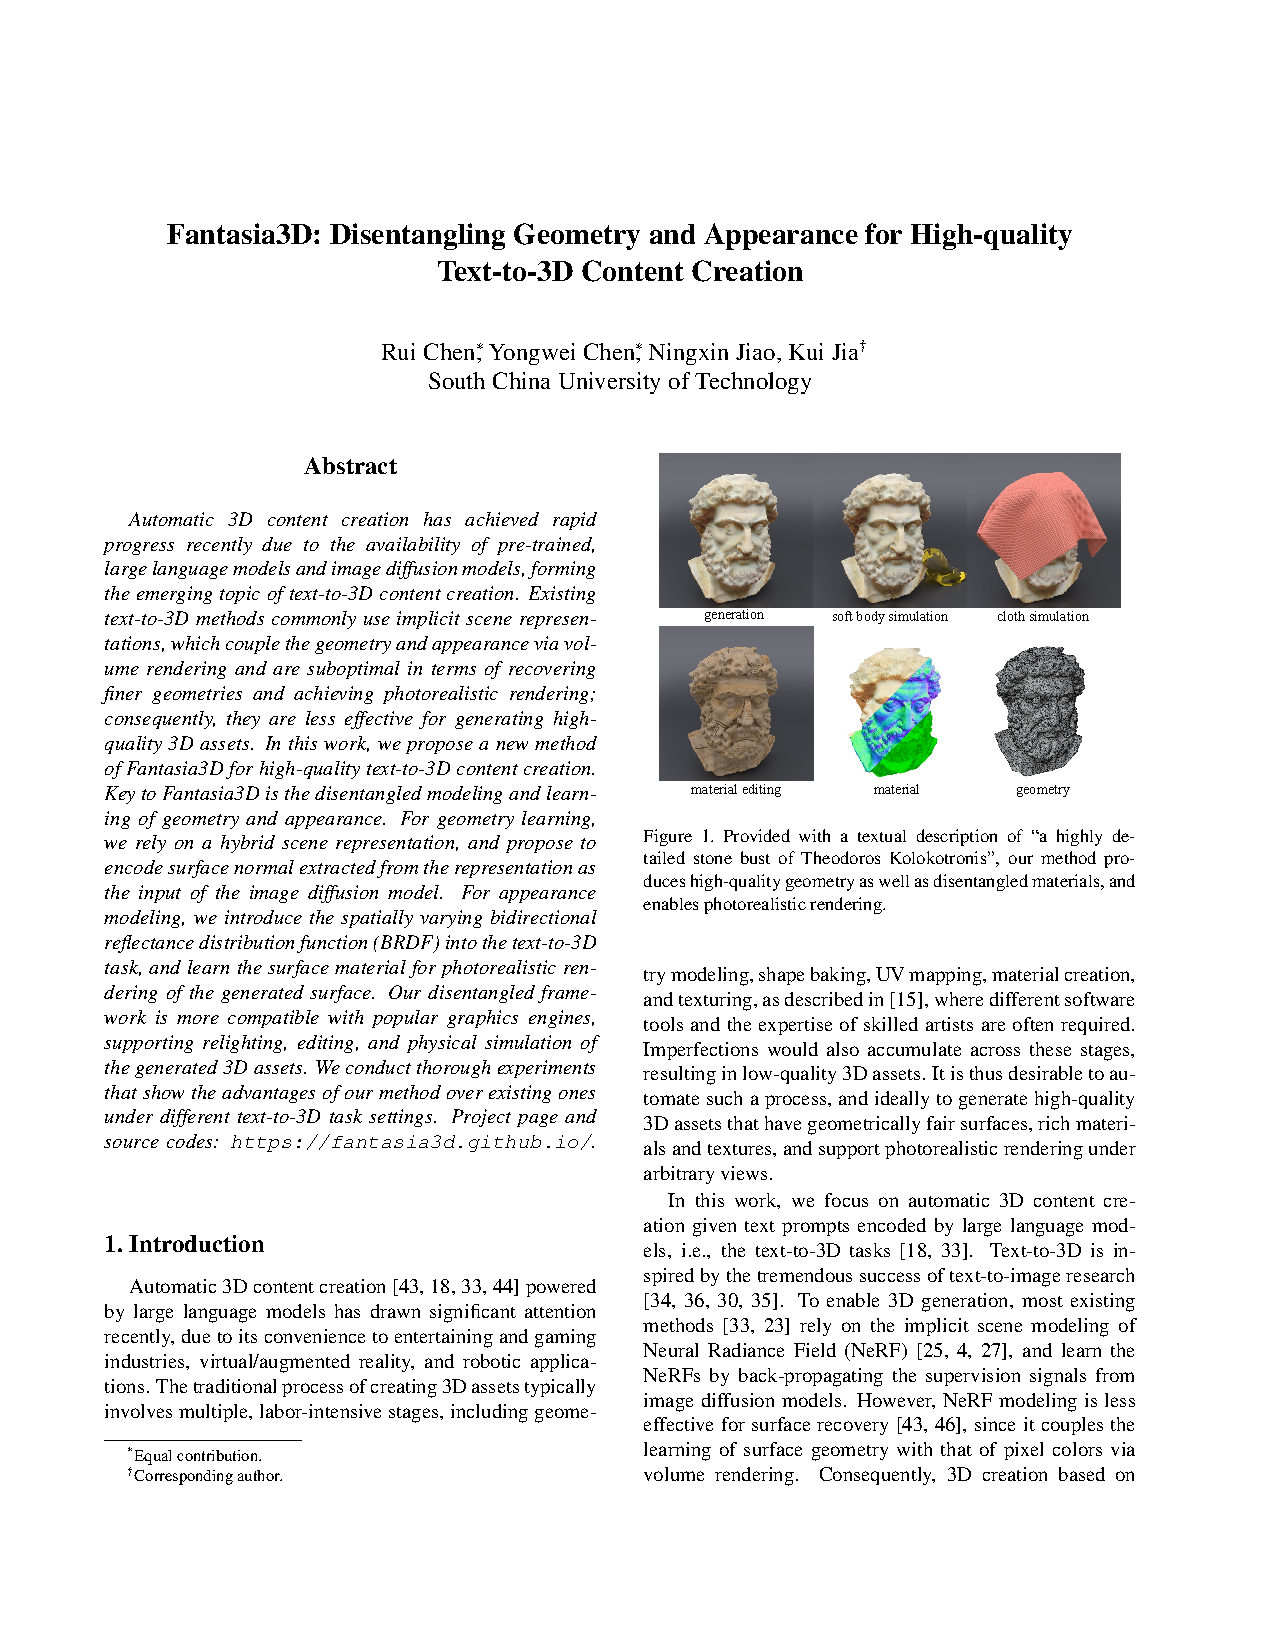
\includegraphics[width=1\columnwidth]{figures/Fantasia3D.png}
      \caption{Outline of the method Fantasia3D. Figure taken From \citep{chen2023fantasia3d}}\label{fig:figureFantasia}
\end{figure}

The geometry stage of Fantasia3D releis on a DMTet which paramererizes the 3D geometry as an MLP\@. 
In the first steps of geometry modeling, Fantasia3D renders and encodes surface normals and the object masks extracted from DMTet, while in the later stages only the rendered normal map is used for the shape encoding \citep{chen2023fantasia3d}. The default initialisation of the DMTet is an ellipsoid, while the model also accepts custom input allowing for more flexibility.  


Appearance Modeling trains another MLP which applies Bidirectional Reflectance Distribution Function (BRDF) on a learned DMTet, ``that predicts parameters of surface material and supports high-qualits 3D generation via photorealistic rendering'' \citep{chen2023fantasia3d}. This function uses the diffuse value \(\text{k}_d\), roughness and metallic \(\text{k}_{rm}\) and normal variation \(\text{k}_n\) in order to apply shading to the geometry. Then, an image is rendered along every ray and the loss is determined using SDS in order tu update the models parameters.    


Both geometry and appearance MLPs are learned through a pre-trained stable diffusion model \citep{rombachStableDiffusion} using Score Distillation Sampling (SDS) loss. 


Fantasia3D allows additional user inputs such as customized 3D shapes or generic 3D shapes of specific categories. This flexibility enhances user control over the content generation process. The disentangled generation of geometry and appearance makes the method compatible with popular graphics engines, supporting relighting, editing, and physical simulation of the generated 3D assets.

While Fantasia3D shows promise in generating photorealistic 3D assets from text, it faces challenges in generating loose geometries like hair, fur, and grass. Additionally, it primarily focuses on object generation, lacking the capacity to create complete scenes with backgrounds from text prompts. Future research aims to address these limitations.

\subsection{Magic 3D}
\label{Magic3D}

Shap-E involves training an encoder which "produces a latent representation of a 3D asset" \citep{junShapeE}. In a second step, a diffusion prior on the obtained latent representations is trained, conditioning it on images or text descriptions to capture additional information \citep{junShapeE}.

\begin{figure}[ht]
    \centering
      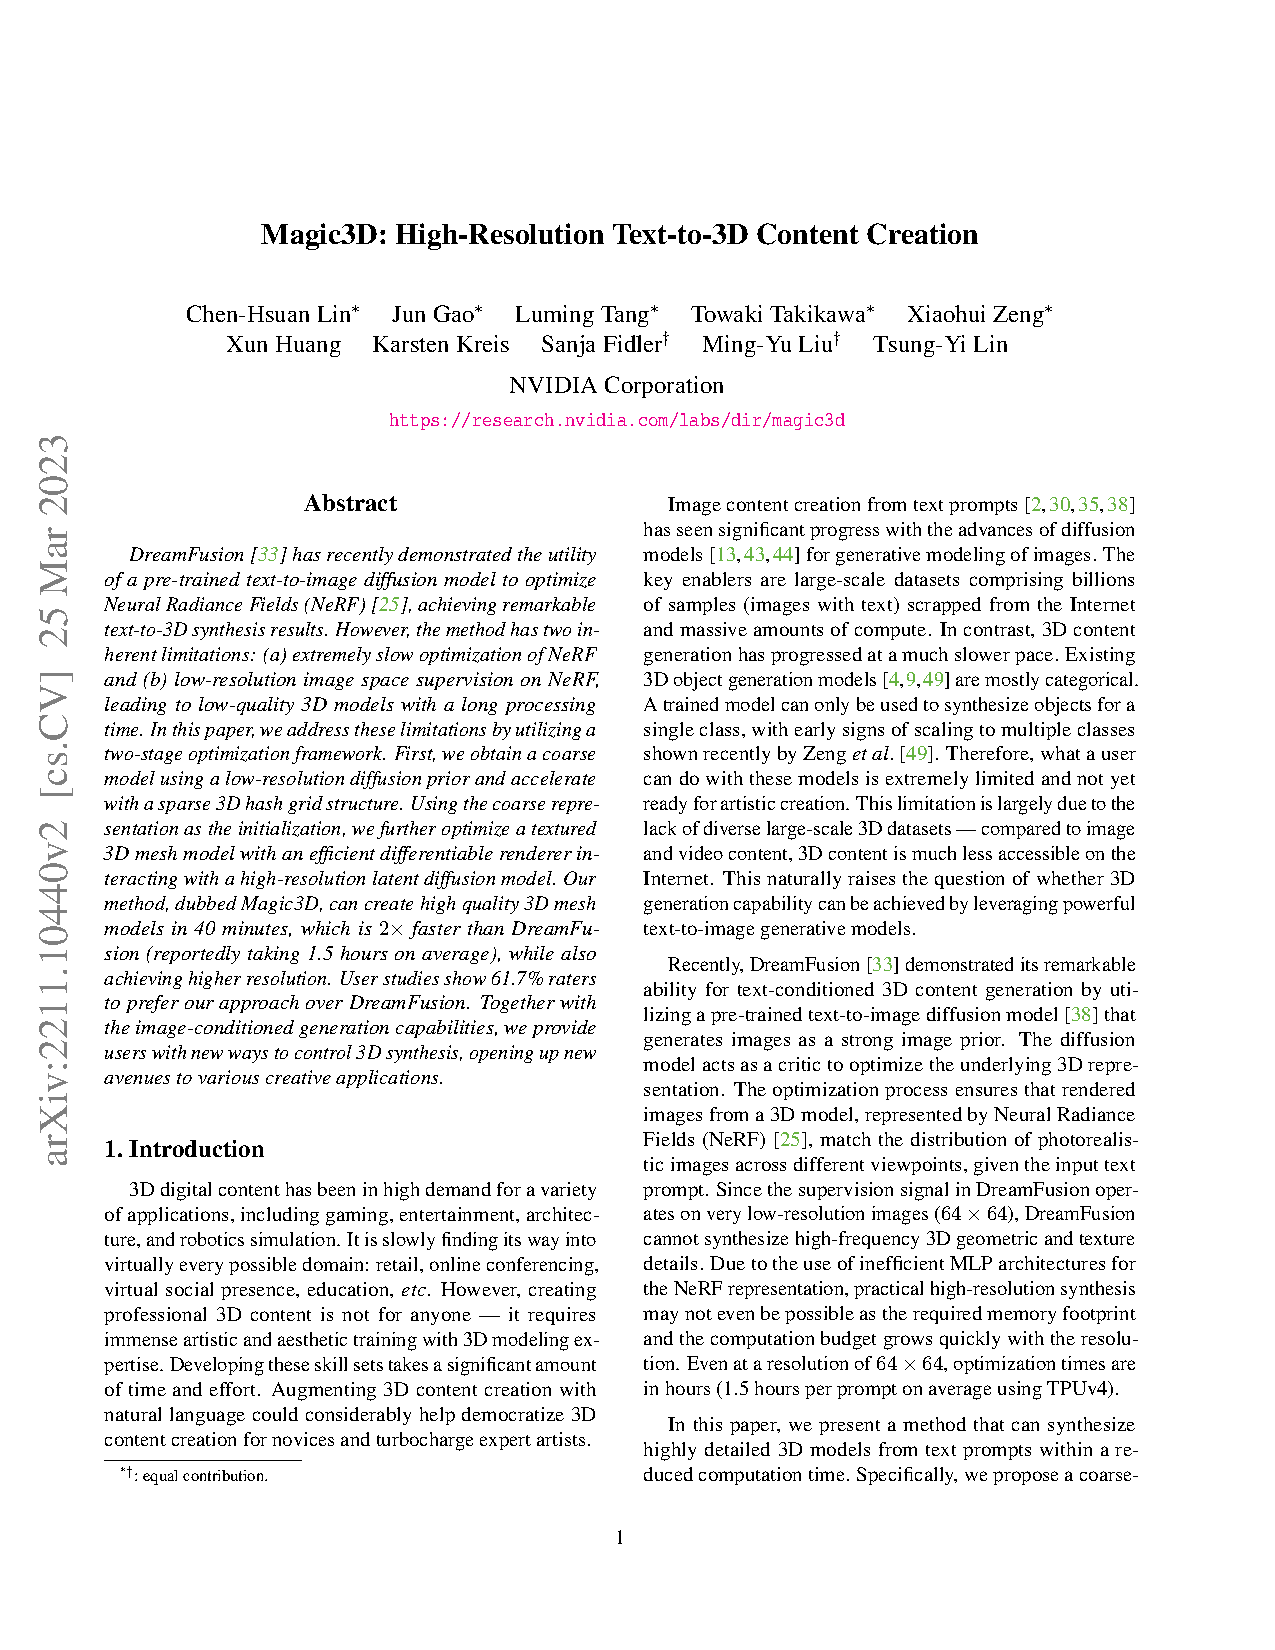
\includegraphics[width=1\columnwidth]{figures/Magic3D.png}
      \caption{Summatized functionality of Magic3D}\label{fig:figureMagic3D}
\end{figure}
